\chapter{Contexte et motivation}

Ce projet s'inscrit dans le cadre du laboratoire de recherche de M.~Antoine Pirog, encadrant du projet R\&D au semestre 7 à Junia. Le laboratoire travaille sur la simulation de réseaux de neurones biophysiques, c'est-à-dire des modèles qui reproduisent le comportement électrique de populations de neurones interconnectés.

Le problème auquel ce type de recherche fait face est simple : la simulation de réseaux de neurones réalistes est coûteuse en temps de calcul. Sur \textbf{CPU}, un réseau de quelques milliers de neurones peut prendre des heures à simuler. Cela limite la taille des réseaux qu'on peut étudier, et donc les questions scientifiques qu'on peut explorer.

Junia dispose de serveurs équipés de cartes graphiques \textbf{RTX~5090}. La question posée est donc : ces \textbf{GPU} peuvent-ils apporter la puissance de calcul nécessaire pour rendre la simulation de grands réseaux de neurones tractable au quotidien pour le laboratoire ?

La réponse n'est pas évidente, et elle n'est pas garantie. Le \textbf{GPU} est théoriquement beaucoup plus puissant, mais notre problème, un système d'\textbf{EDO} couplées avec des connexions irrégulières, n'est pas forcément un cas idéal pour le parallélisme massif. Il est tout à fait possible que la conclusion soit : non, sur ce type de simulation, le \textbf{GPU} n'apporte pas un gain suffisant pour justifier le changement d'architecture. Le but du projet est d'apporter une réponse documentée et mesurée à cette question, pas d'arriver à une conclusion prédéterminée.

C'est dans ce contexte que le sujet \og Optimisation de modèles neuronaux à oscillateurs couplés \fg{} nous a été confié, avec un socle de code déjà existant : modèle de \textbf{Hodgkin-Huxley}, \textbf{synapses}, solveur \textbf{CPU} de référence. On part de cette base pour évaluer l'intérêt du \textbf{GPU}.

\chapter{Présentation du sujet}

\section{Énoncé et objectif}

Ce projet a pour objectif d'évaluer la faisabilité de l'utilisation des architectures \textbf{GPU} pour la simulation de réseaux de neurones. Il s'agit de déterminer la capacité maximale du système en nombre de \textbf{synapses} prises en charge, tout en précisant les conditions dans lesquelles le calcul sur \textbf{GPU} surpasse une exécution sur \textbf{CPU}. Enfin, les travaux visent à accélérer et à optimiser les performances de simulation en s'appuyant sur nos compétences techniques.

L'approche suivie s'articule en cinq étapes : modélisation \textbf{Hodgkin-Huxley}, couplage par \textbf{synapses}, construction d'un \textbf{connectome}, portage sur \textbf{GPU}, puis \textbf{benchmark} \textbf{CPU}/\textbf{GPU}. L'objectif final est de produire une courbe de \textbf{speedup} en fonction de la taille du réseau, qui montre à partir de quel nombre de neurones le \textbf{GPU} devient indispensable, et dans quelle mesure il l'est.

\section{Le modèle de Hodgkin-Huxley}

Le socle de code fourni repose sur le modèle de \textbf{Hodgkin-Huxley}. Il s'agit d'une modélisation biologique dans laquelle un neurone est assimilé à un circuit électrique, simulant l'activité cérébrale à partir du flux d'ions sodium et potassium. Le modèle décrit l'évolution du \textbf{potentiel membranaire} par un système d'équations différentielles ordinaires (\textbf{EDO}) gouvernant l'ouverture et la fermeture des \textbf{canaux ioniques}. C'est ce formalisme, une \textbf{EDO} par neurone répétée sur l'ensemble du réseau, qui rend le problème naturellement parallélisable.

\section{Problématique}

\textbf{Problématique.} Comment accélérer la simulation de réseaux de neurones de \textbf{Hodgkin-Huxley} couplés lorsque la taille du \textbf{connectome} augmente, et quelle stratégie \textbf{GPU} offre le meilleur gain par rapport à la référence \textbf{CPU}, à résultats équivalents ?

\textbf{La vraie question du projet.} Le laboratoire de M.~Pirog peut-il, grâce aux serveurs Junia équipés de \textbf{RTX~5090}, simuler des réseaux de neurones assez grands pour être utiles à la recherche, dans un temps acceptable ?

\begin{figure}[p]
\centering
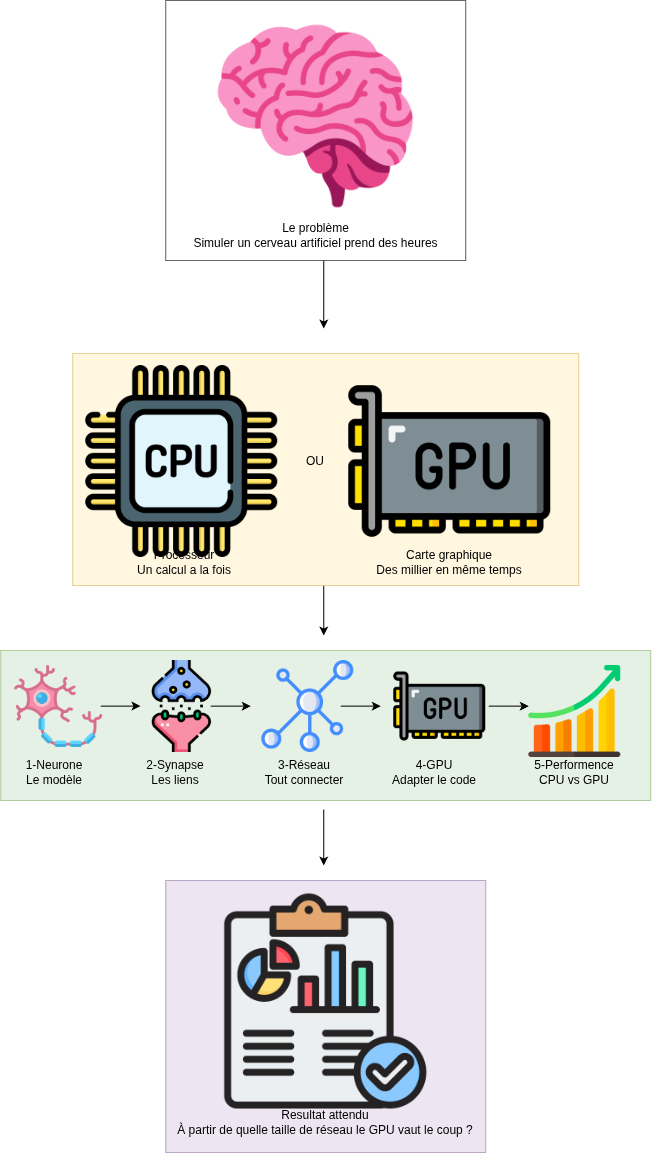
\includegraphics[height=0.92\textheight]{Shema_livrable1.png}
\caption{Carte conceptuelle du projet : qui, quoi, comment, pourquoi, enjeux et contraintes.}
\end{figure}

